\begin{figure}[t!]
\vspace{-14pt}
\begin{singlespace}
\hfill
\begin{minipage}{2.2in}
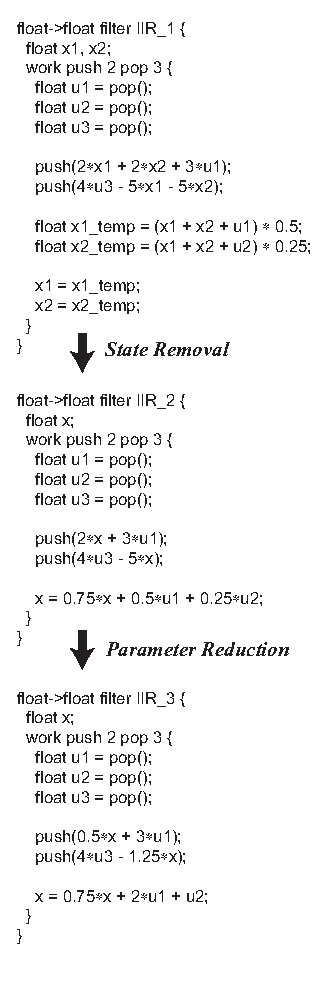
\epsfig{file=statespace-example.eps, width=2.05in}
\end{minipage}
~~~~
\raisebox{10pt}{
\begin{minipage}{3.5in}
\vspace{10pt}
{\small
Number of multiplications: 8 \\
Number of additions: 8 \\
State space representation:
}
\begin{eqnarray*}
\small
\vec{\mathbf{y}} & = & \left [ \begin{array} {cc} 2 & 2 \\ -5 & -5
\end{array} \right ] \vec{\mathbf{x}} + \left [ \begin{array} {ccc} 3 & 0 & 0 \\ 0 & 0 & 4 \end{array} \right
 ] \vec{\mathbf{u}} \\
\vec{\dot{\mathbf{x}}} & = & \left [ \begin{array} {cc} 0.5 & 0.5 \\ 0.25
& 0.25 \end{array} \right ] \vec{\mathbf{x}} + \left [ \begin{array} {ccc} 0.5 & 0 & 0 \\
0 & 0.25 & 0 \end{array} \right ] \vec{\mathbf{u}}
\end{eqnarray*}
\vspace{-3pt} ~ \\
\hrule
\vspace{26pt} ~ \\
{\small
Number of multiplications: 7 \\
Number of additions: 4 \\
State space representation:}
\begin{eqnarray*}
\small
\vec{\mathbf{y}} & = & \left [ \begin{array} {cc} 2 \\ -5
\end{array} \right ] \vec{\mathbf{x}} + \left [ \begin{array} {ccc} 3 & 0 & 0 \\ 0 & 0 & 4 \end{array} \right
 ] \vec{\mathbf{u}} \\
\vec{\dot{\mathbf{x}}} & = & \left [ \begin{array} {cc} 0.75
\end{array} \right ] \vec{\mathbf{x}} + \left [ \begin{array} {ccc} 0.5 & 0.25 & 0 \end{array} \right ] \vec{\mathbf{u}}
\end{eqnarray*}
\hrule
\vspace{12pt} ~ \\
{\small
Number of multiplications: 5 \\
Number of additions: 4 \\
State space representation:}
\begin{eqnarray*}
\small
\vec{\mathbf{y}} & = & \left [ \begin{array} {cc} 1 \\ -2.5
\end{array} \right ] \vec{\mathbf{x}} + \left [ \begin{array} {ccc} 3 & 0 & 0 \\ 0 & 0 & 4 \end{array} \right
 ] \vec{\mathbf{u}} \\
\vec{\dot{\mathbf{x}}} & = & \left [ \begin{array} {cc} 0.75
\end{array} \right ] \vec{\mathbf{x}} + \left [ \begin{array} {ccc} 1 & 0.5 & 0 \end{array} \right ] \vec{\mathbf{u}}
\end{eqnarray*}
\end{minipage}}
\end{singlespace}
\begin{center}
\vspace{-24pt}
\caption{Example optimization of an IIR filter using linear state
space analysis.  The top segment shows the original code.  The middle
segment depicts the action of state removal, in which the quantity
$x_1 + x_2$ is replaced by a single variable $x$.  The bottom segment
illustrates parameter reduction, in which the coefficients are
refactored to eliminate two multiplications (two coefficients
assume a value of 1).\protect\label{fig:opt-seq}}
\end{center}
\vspace{-18pt}
\hrule
\vspace{-12pt}
\end{figure}
